\subsubsection{\newtext{Exploration Time}}
\label{subsubsec:overall-time}

\begin{figure}[h]
\vspace{-8pt}
	\centering
		\subfloat[OpenVX: Diff \#ACCs] {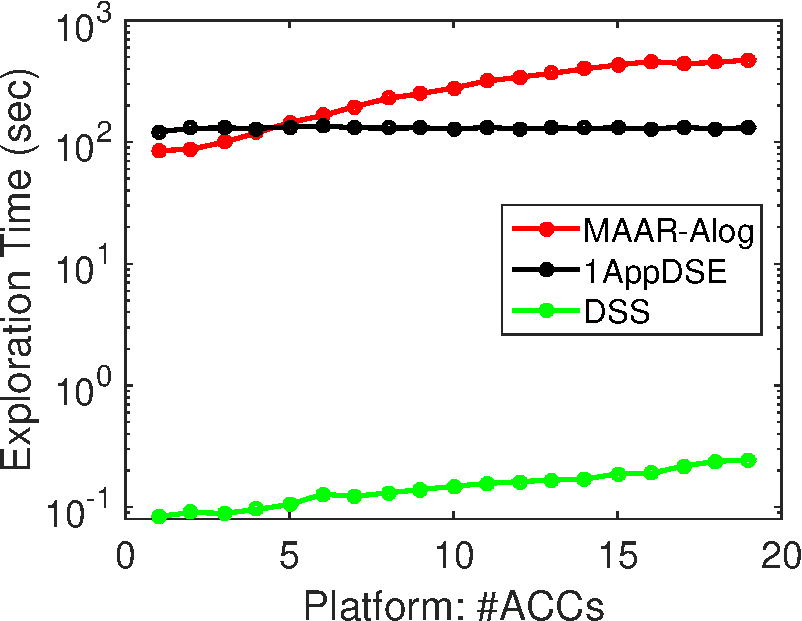
\includegraphics[width=.48\linewidth]{fig/timeACCs_all.pdf}\label{fig:timeACCs_all}}
		\hfill
		\subfloat[Synthetic: Diff \#Apps] {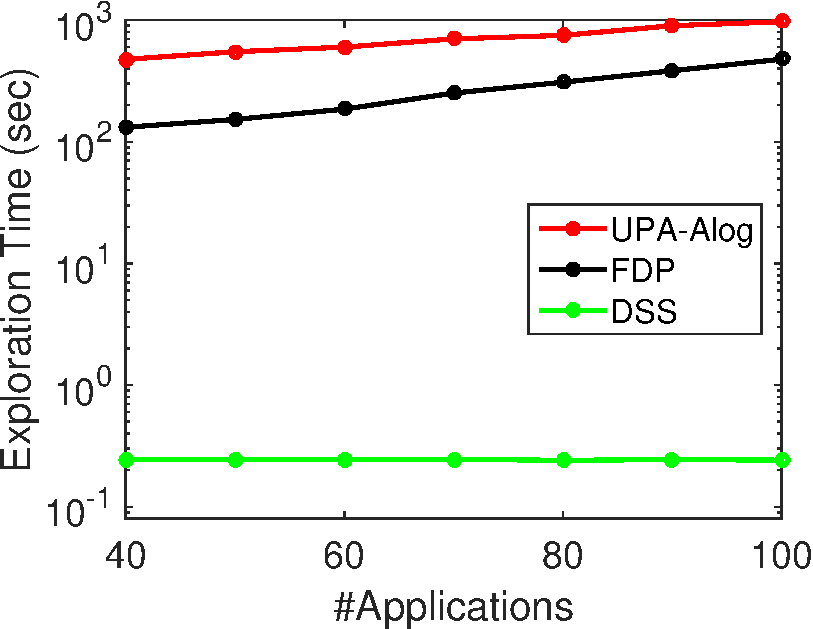
\includegraphics[width=.48\linewidth]{fig/timeApps_all.pdf}\label{fig:timeApps_all}}
	\vspace{-8pt}
	\caption{Exploration Time}
	\label{fig:exTime_all}
\end{figure}

\newtext{
\figref{fig:exTime_all} shows the exploration time of different DSEs running on Intel i5-3450 with 3.10GHz.
\figref{fig:timeACCs_all} demonstrates the exploration time for OpenVX applications with an increasing ACC budget. Both DSS and MAAR exploration time increases, because the platform design space gets bigger with the increasing number of ACCs. From ACCs=1 to ACCs=19, DSS's exploration time increases from 0.084 seconds to 0.245 seconds, and MAAR is from 85.10 seconds to 475.56 seconds. DSS is much faster than MAAR, since DSS is only a greedy selection algorithm and MAAR contains a large number of evaluations. 
1AppDSE, which is an exhaustive search for each application, has an almost constant exploration time because it only contains DSE for the individual application, which has a small design space with less size changing. With the ACC increasing, the individual application design space does not increase much, because the number of unique kernels (ACC candidates) is only 2-9, while there are 35 kernels in many applications. 

\figref{fig:timeApps_all} shows the exploration time versus an increasing number of applications using synthetically generated applications. The total number of unique kernels in all application sets are 35, and DSEs explore platform(s) with a budget ACCs=19. 
The DSS exploration time is almost constant around 0.245 seconds, because it selects ACC using profiled characteristics from applications, and the number of applications does not impact on the exploration \cite{zhang2018ds}.
With increasing applications from 40 to 100, MAAR exploration time increases from 475.56 seconds to 971.26 seconds, because it contains an increasing number of individual applications evaluation for each platform candidate.
Similarly, 1AppDSE exploration time increases significant from 131.65 seconds to 477.75 seconds, because of more DSE problems for individual application.   
}